\section{Illustrative Scenario}\label{sec:scenarios}
We illustrate an application of {\sc GeoHighlight} in a realistic scenario for New York taxi dataset\footnote{\it http://www.nyc.gov/html/tlc/html/about/trip_record_data.shtml}. We consider 100,000 unique points of this dataset. The following scenario illustrates how an analyst can achieve an analysis goal in her mind. We employ {\sc Highlighter} (Algorithm \ref{algo:geoh}) to obtain results of the scenario with following parameters: $\sigma = 0.2$, $k = 5$ and $tlimit = 200ms$. 

\vspace{5pt}
\noindent {\bf Dataset Description.} [Here, we briefly describe the New York tax dataset (statistics and attributes)]

\begin{figure}
  \centering
  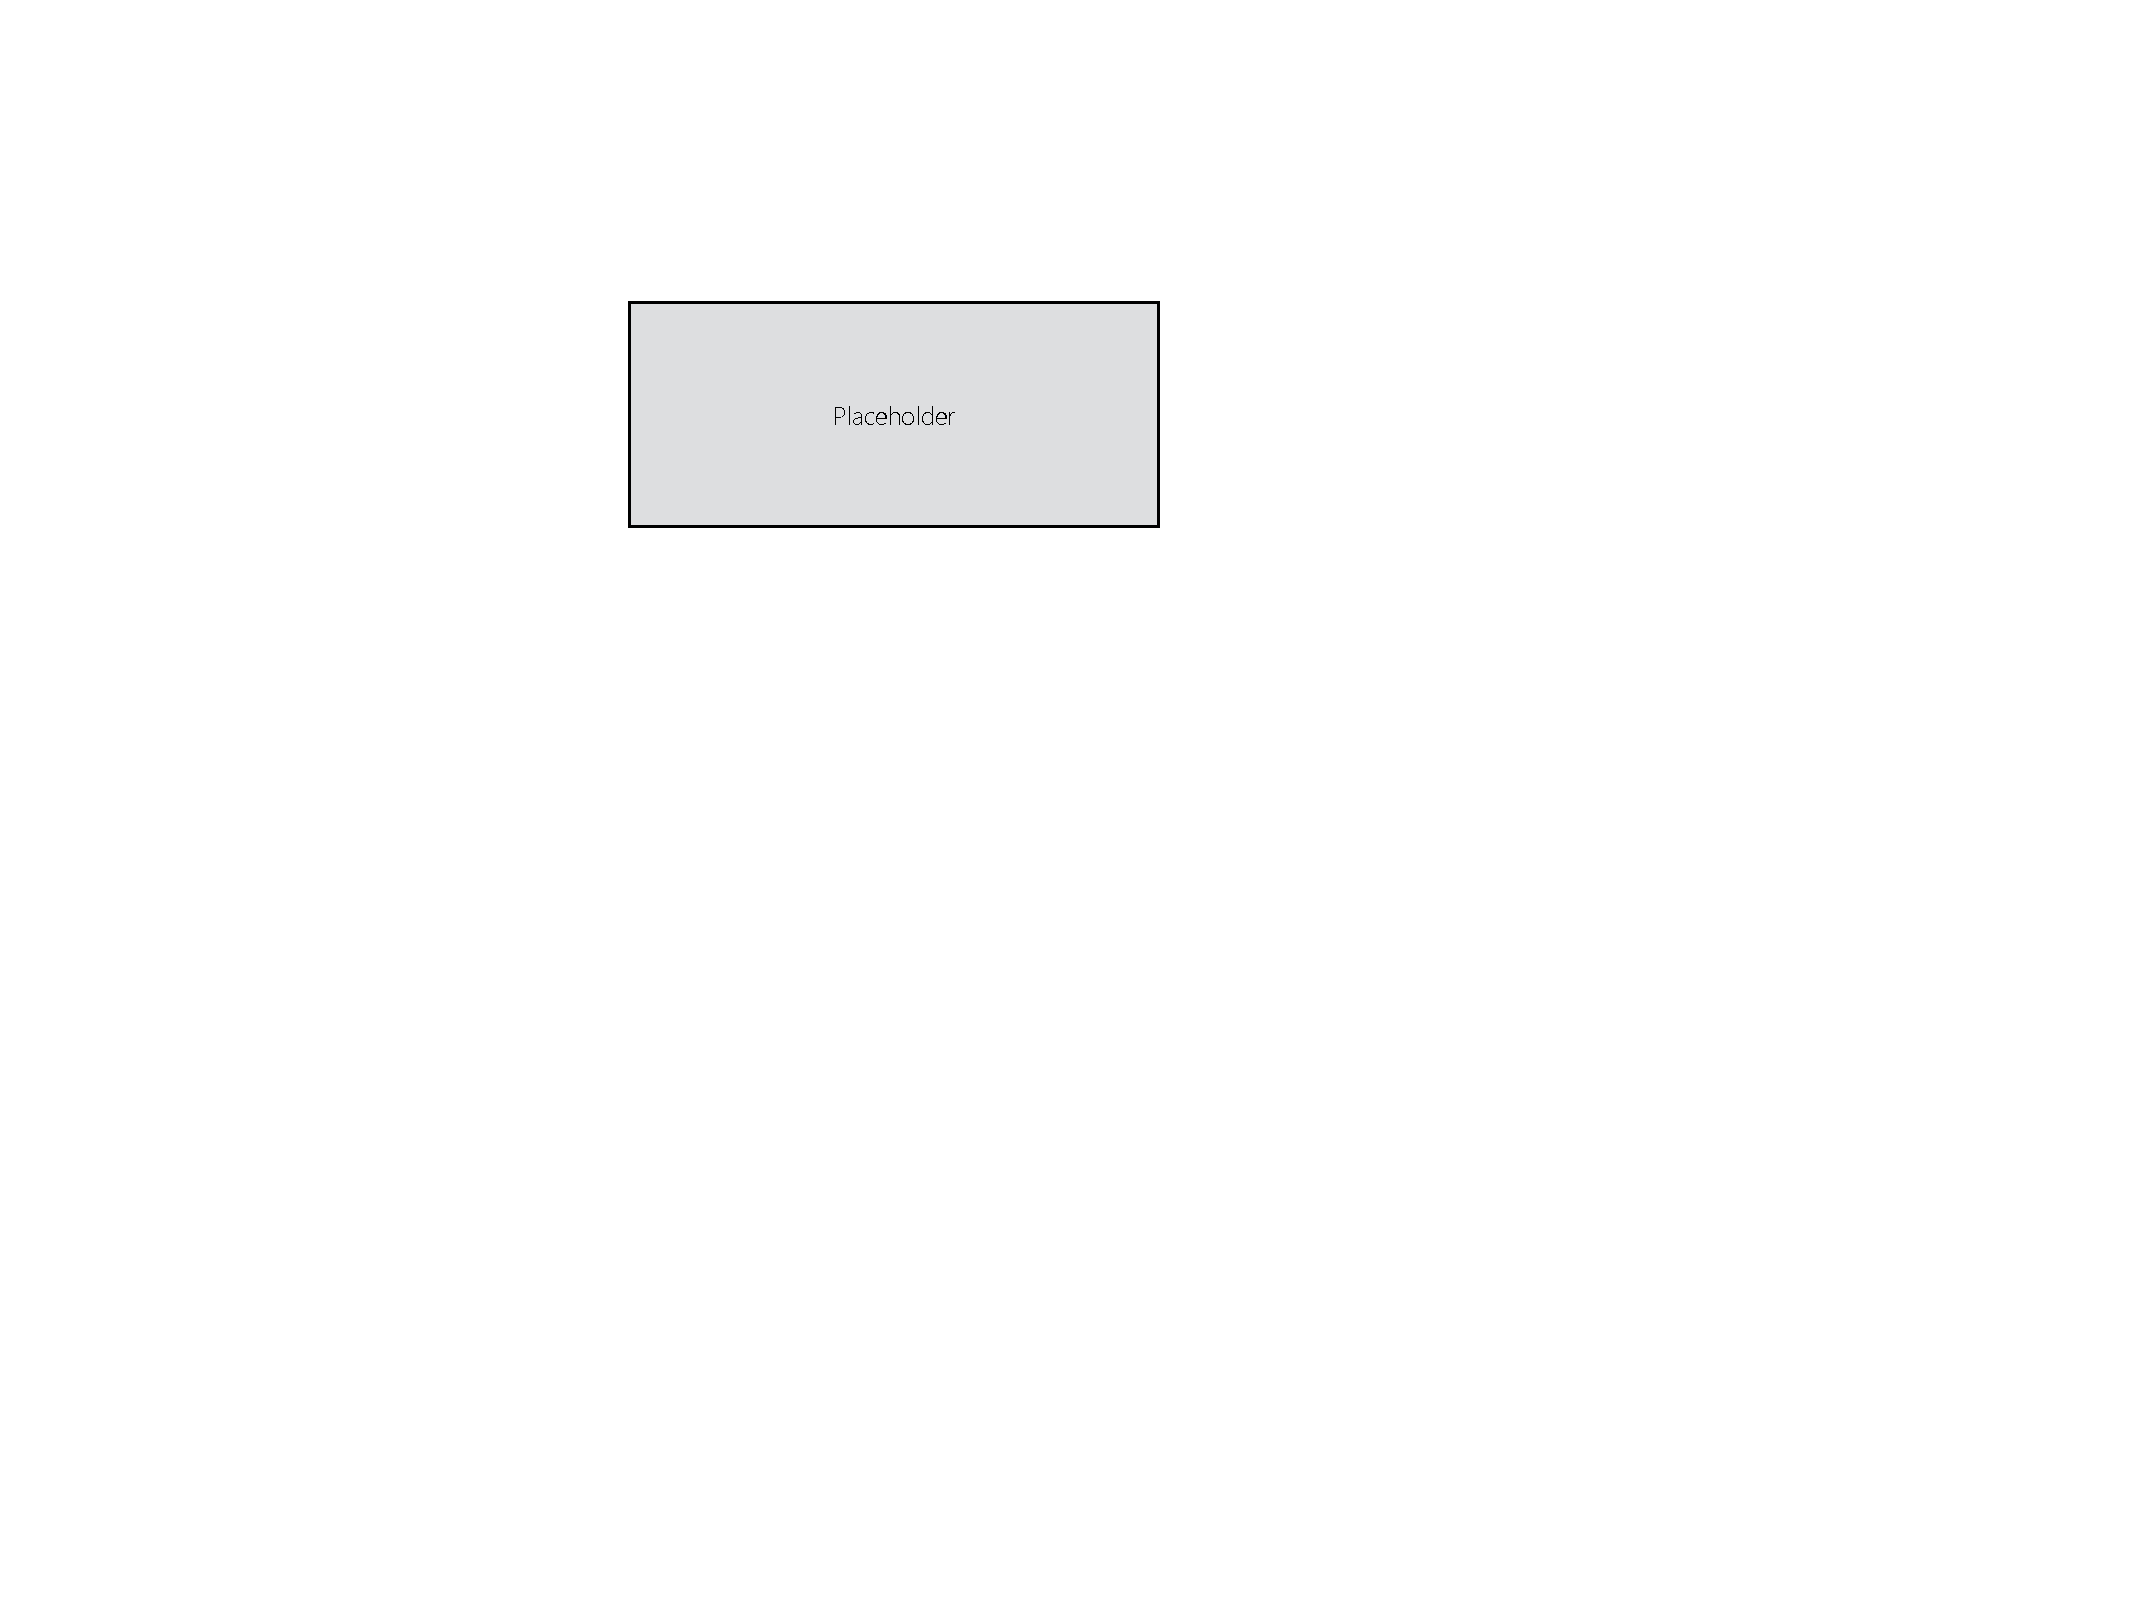
\includegraphics[width=\columnwidth]{figs/placeholder}
\caption{Application of {\sc GeoHighlight} on New York Taxi dataset}
\label{fig:app}
\end{figure}

\vspace{5pt}
Consider Lucas, a data scientist whose task is to optimize New York taxi trips. Focusing on cab-idle locations, he wants to discover which neighborhoods work the best for which drivers to increase the overall availability. Also, he wants to discover how next cab-idle stations should be chosen to contribute to the goal. Lucas uses {\sc GeoHighlight} and follows a case-by-case inspection as his analysis methodology.

He begins the analysis by selecting a point from the most crowded region of the region, i.e., Times Square. The selected point depicts a drop-off at [date/time]. {\sc Highlighter} then provides $5$ relevant points to the selected point (Figure \ref{fig:app}). These highlights show similar points to the selection in other neighborhoods of the region. Among 5 highlighted points, Lucas then selects the 3rd one, a pick-up at [date/time] because [reason based on observation].

Then in the next step, {\sc Highlighter} shows 5 other points relevant to the new selection. This new result show how drop-offs in [location] relate to neighbor locations and how next can-idle sop can be chosen. Lucas selects the first highlighted point [reason based on observation].